\chapter{Evaluation}

\section{Customer Requirements}

In this section I will evaluate whether I have fulfilled each objective which were set in my system specifications. This will determine whether the system meets the full customer requirements. Where the objectives may not have been met, I will evaluate and explain the reason for this being so. I will also provide evidence to prove that objectives have been met in other cases, which will determine that the system has acheived its specifications

%include as many subsections as necessary for your objectives
\subsection{Objective Evaluation}

%from analysis
The general objectives are:
\begin{itemize}
    \item Organised layout for the database.
    \item Prevention of unnecessary duplication of data.
    \item Simple interface for entering data, meaning it can be conducted quickly.
    \item Search function to find a specific customer in the database.
    \item Ability to edit existing data easily and quickly.
    \item Ability to calculate royalties using given data
\end{itemize}

\underline{Objective: Organised layout for the database}

This objective has been fulfilled by clearly labelling each window and giving clear table headings for each table. For example, the customer table clearly shows the following headings: "Author ID", "Firstname", "Lastname", "Email", "Phonenumber", "Address" and "Postcode". This can be seen in Figure \ref{fig:InterfaceClarity} below.

\begin{figure}[H]
    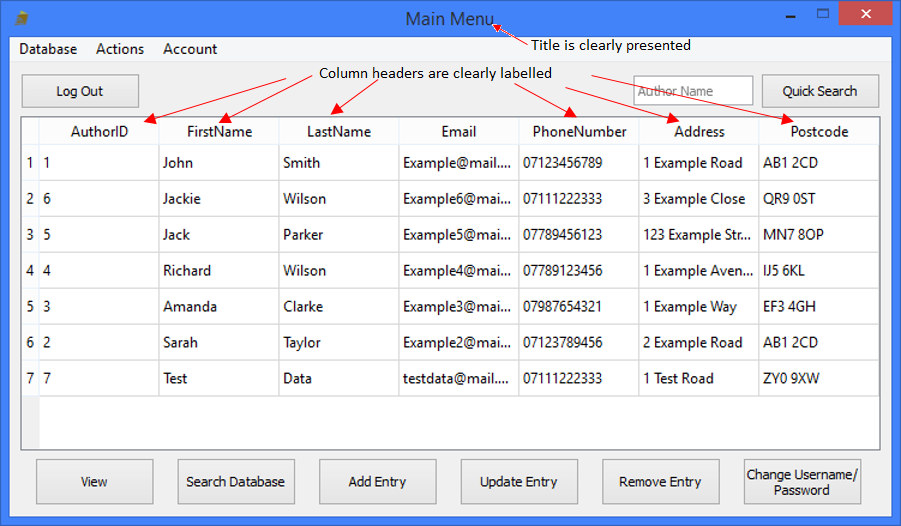
\includegraphics[width=\textwidth]{./Evaluation/Evidence/Clarity.png}
    \label{fig:InterfaceClarity} \caption{Interface is titled and tables are clearly labelled}
\end{figure}

Also, in question 1 of the questionnaire in page \pageref{fig:Questionnaire1}, the client has strongly agreed with the statement in the question and said that the titles on windows make the interface clear to them. The user has said that the large buttons make navigation easy as it is difficult to misclick a button. Furthermore, the headings can be clicked to sort the details by alphabetical order, ascending or descending. The tables each hold data from only 1 entity, so that the user does not get confused with the data in the table.


\underline{Objective: Preventing Duplication}

This objective has not been fulfilled, as the system does not run checks to see whether the data is already existent in the database. The answer to question 12 of the questionnaire, on page \pageref{fig:Questionnaire2} shows that the user disagrees with whether the system prevents unneccessary duplication efficiently. The client has said that the system does not warn the user of the duplication, which proves that the system does not run any of these checks. However, the use of ID's still make each author unique, and the client has said the searches can be easily conducted to check whether the data is existent or not. 


\underline{Objective: Simple interface for entering data, meaning it can be conducted quickly.}

This objective has been fulfilled, as entry boxes are clearly labelled, and there are only as many boxes as required for each entry. The entry boxes are all in line with each other, making it look tidy instead of looking cluttered. This can be seen in Figure \ref{fig:AddingInterface} below.

\begin{figure}[H]
    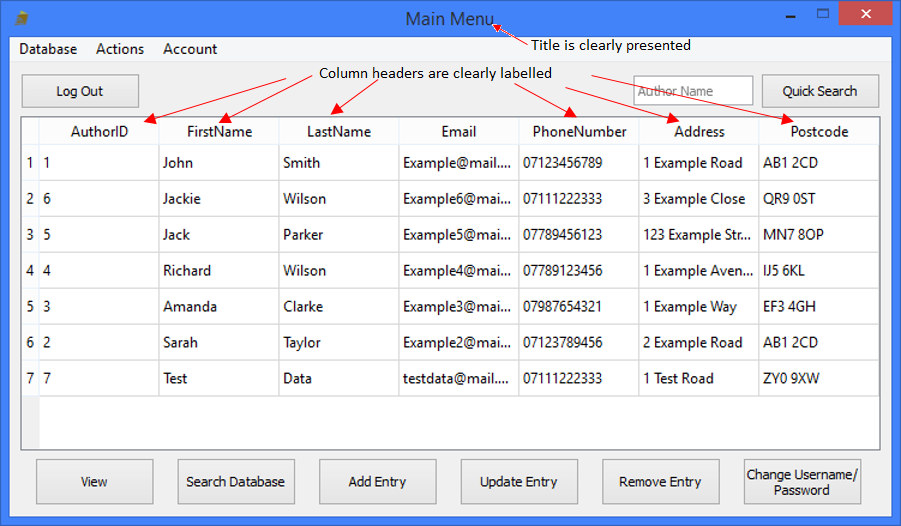
\includegraphics[width=\textwidth]{./Evaluation/Evidence/Clarity.png}
    \label{fig:AddingInterface} \caption{Simple interface for entering data}
\end{figure}

The client has also strongly agreed with questions 2 and 3, which show that they think that there isn't a problem with the interfaces for adding data. Each different interface for adding an certain entry has a specific title to show what is being added, which makes the current entry clear to the user.

\section{Effectiveness}

%include as many subsections as necessary for your objectives
\subsection{Objective Evaluation}

\section{Learnability}

\section{Usability}

\section{Maintainability}

\section{Suggestions for Improvement}

\section{End User Evidence}

\subsection{Questionnaires} 

\begin{figure}[H]
    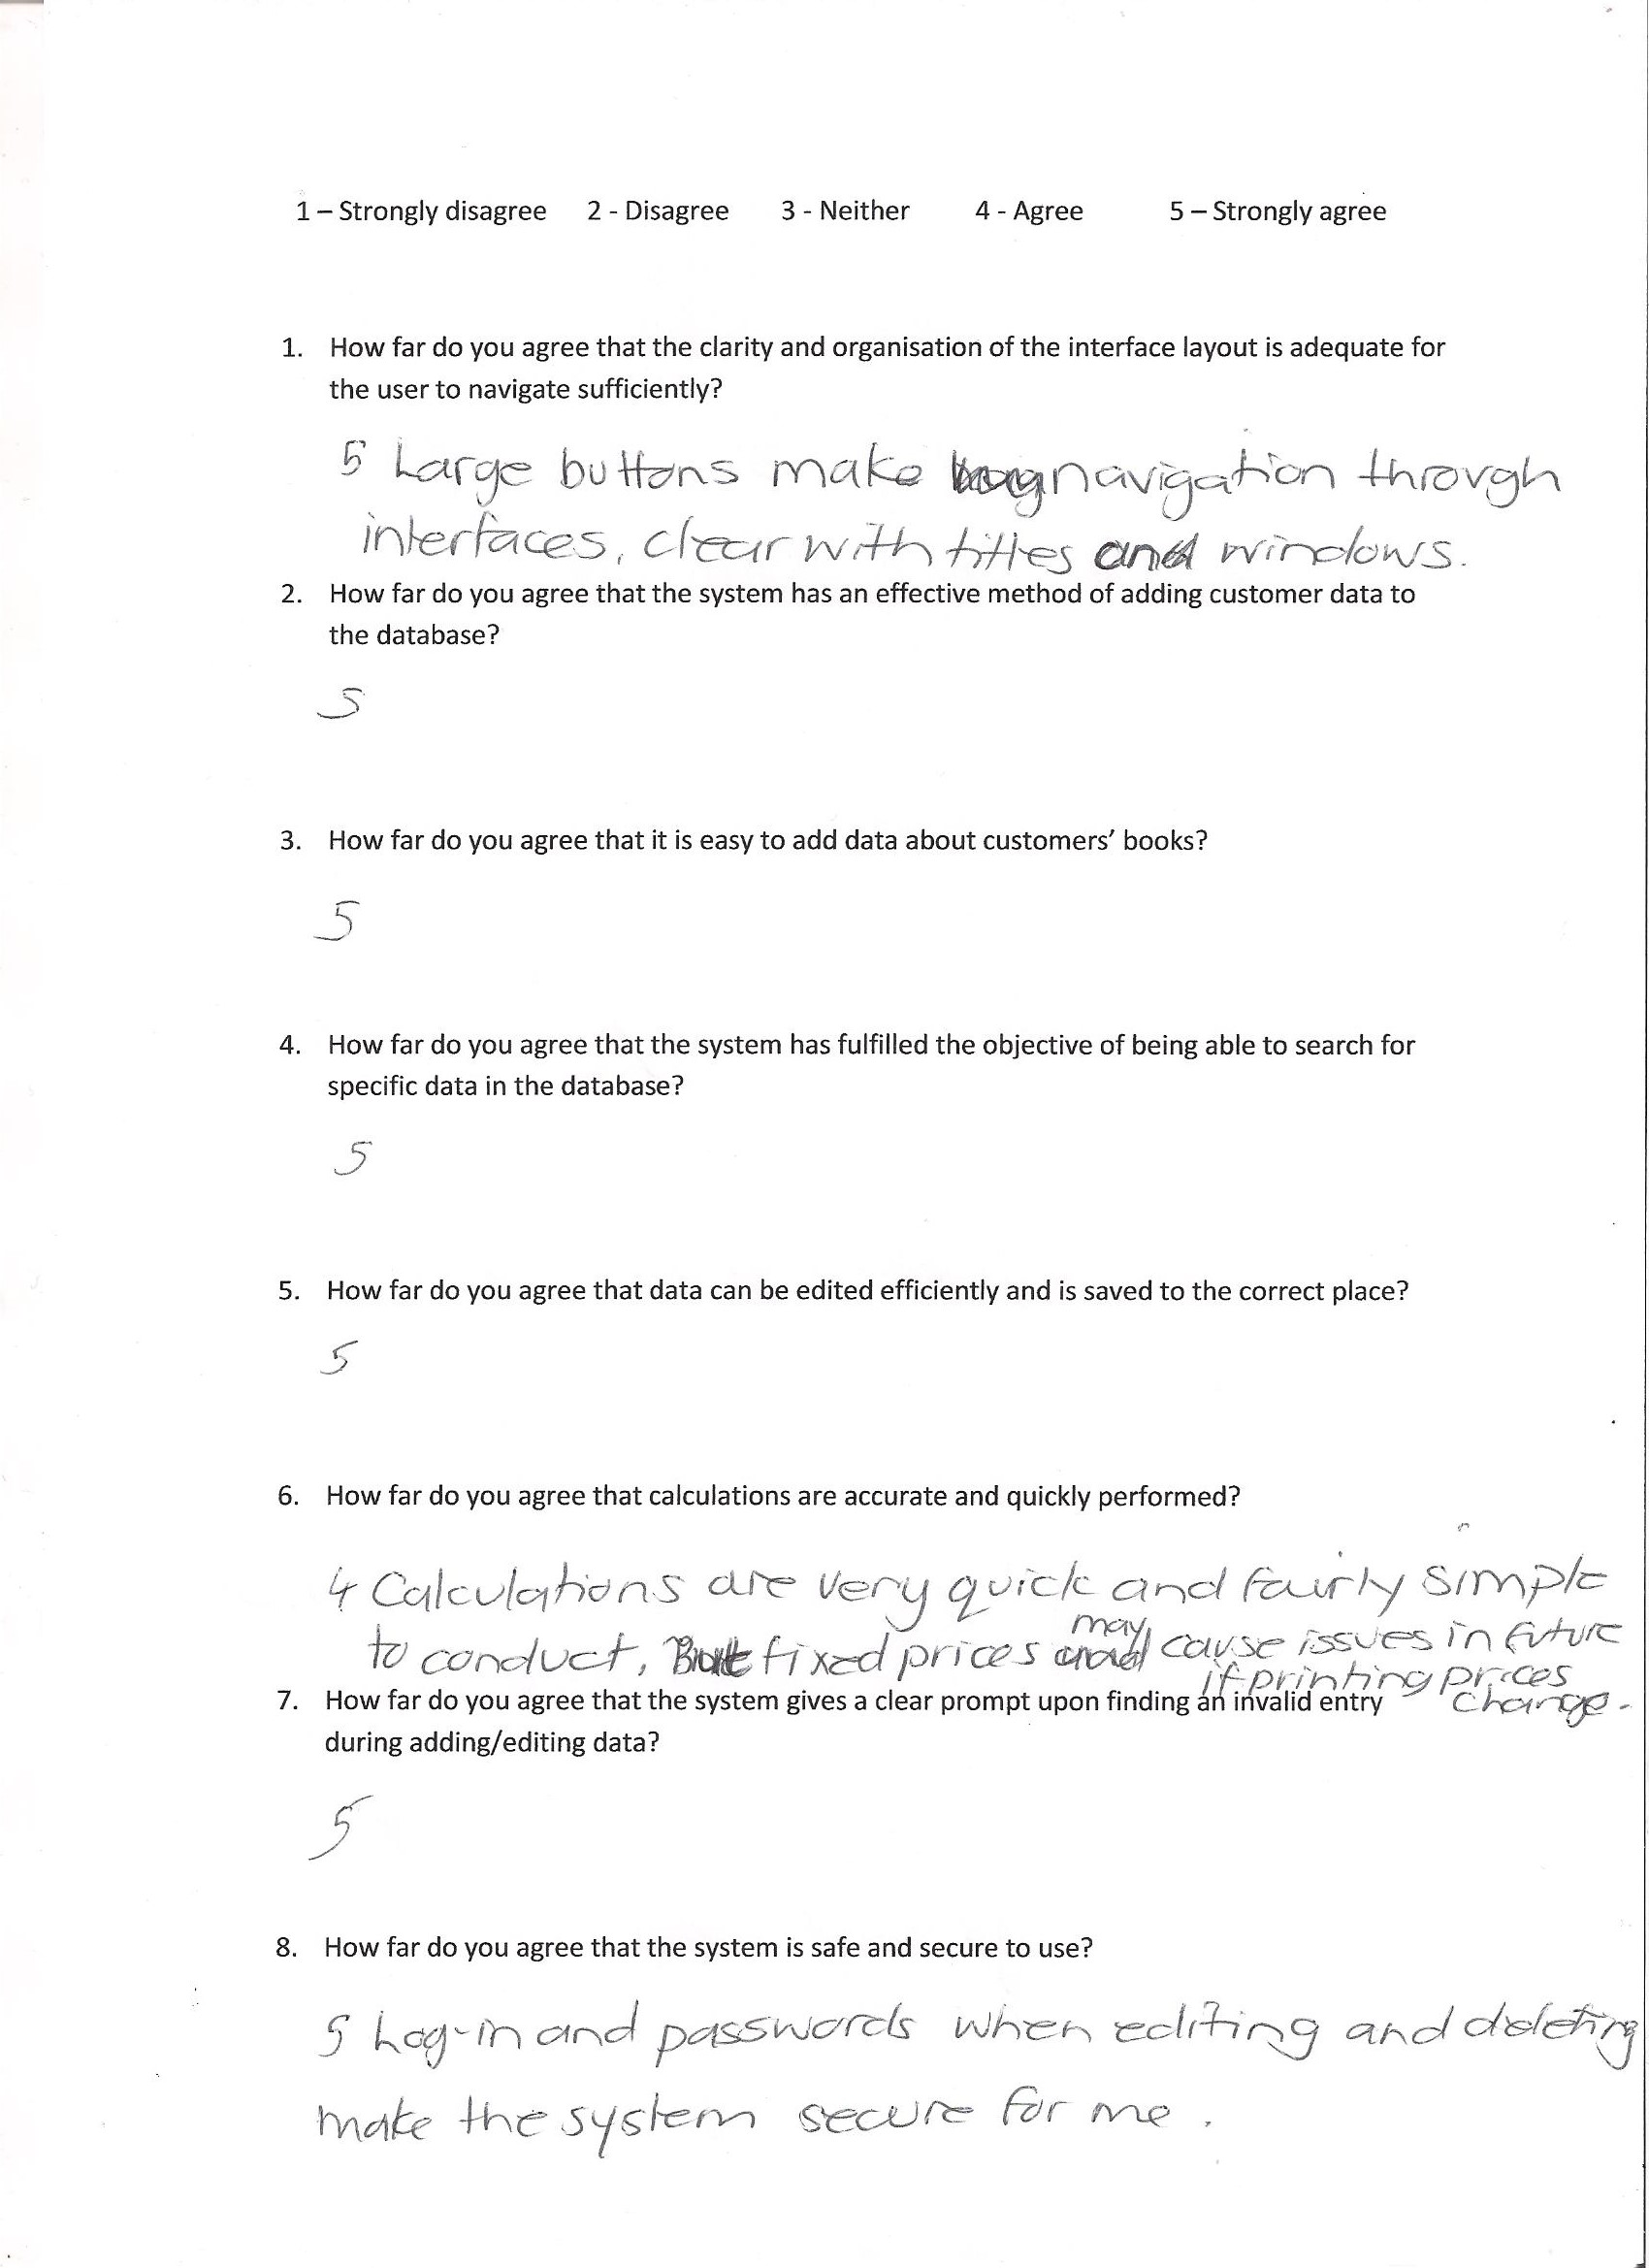
\includegraphics[width=\textwidth]{./Evaluation/Questionnaire1.png}
    \label{fig:QuestionnairePage1} \caption{Page 1 of Questionnaire}
\end{figure}

\begin{figure}[H]
    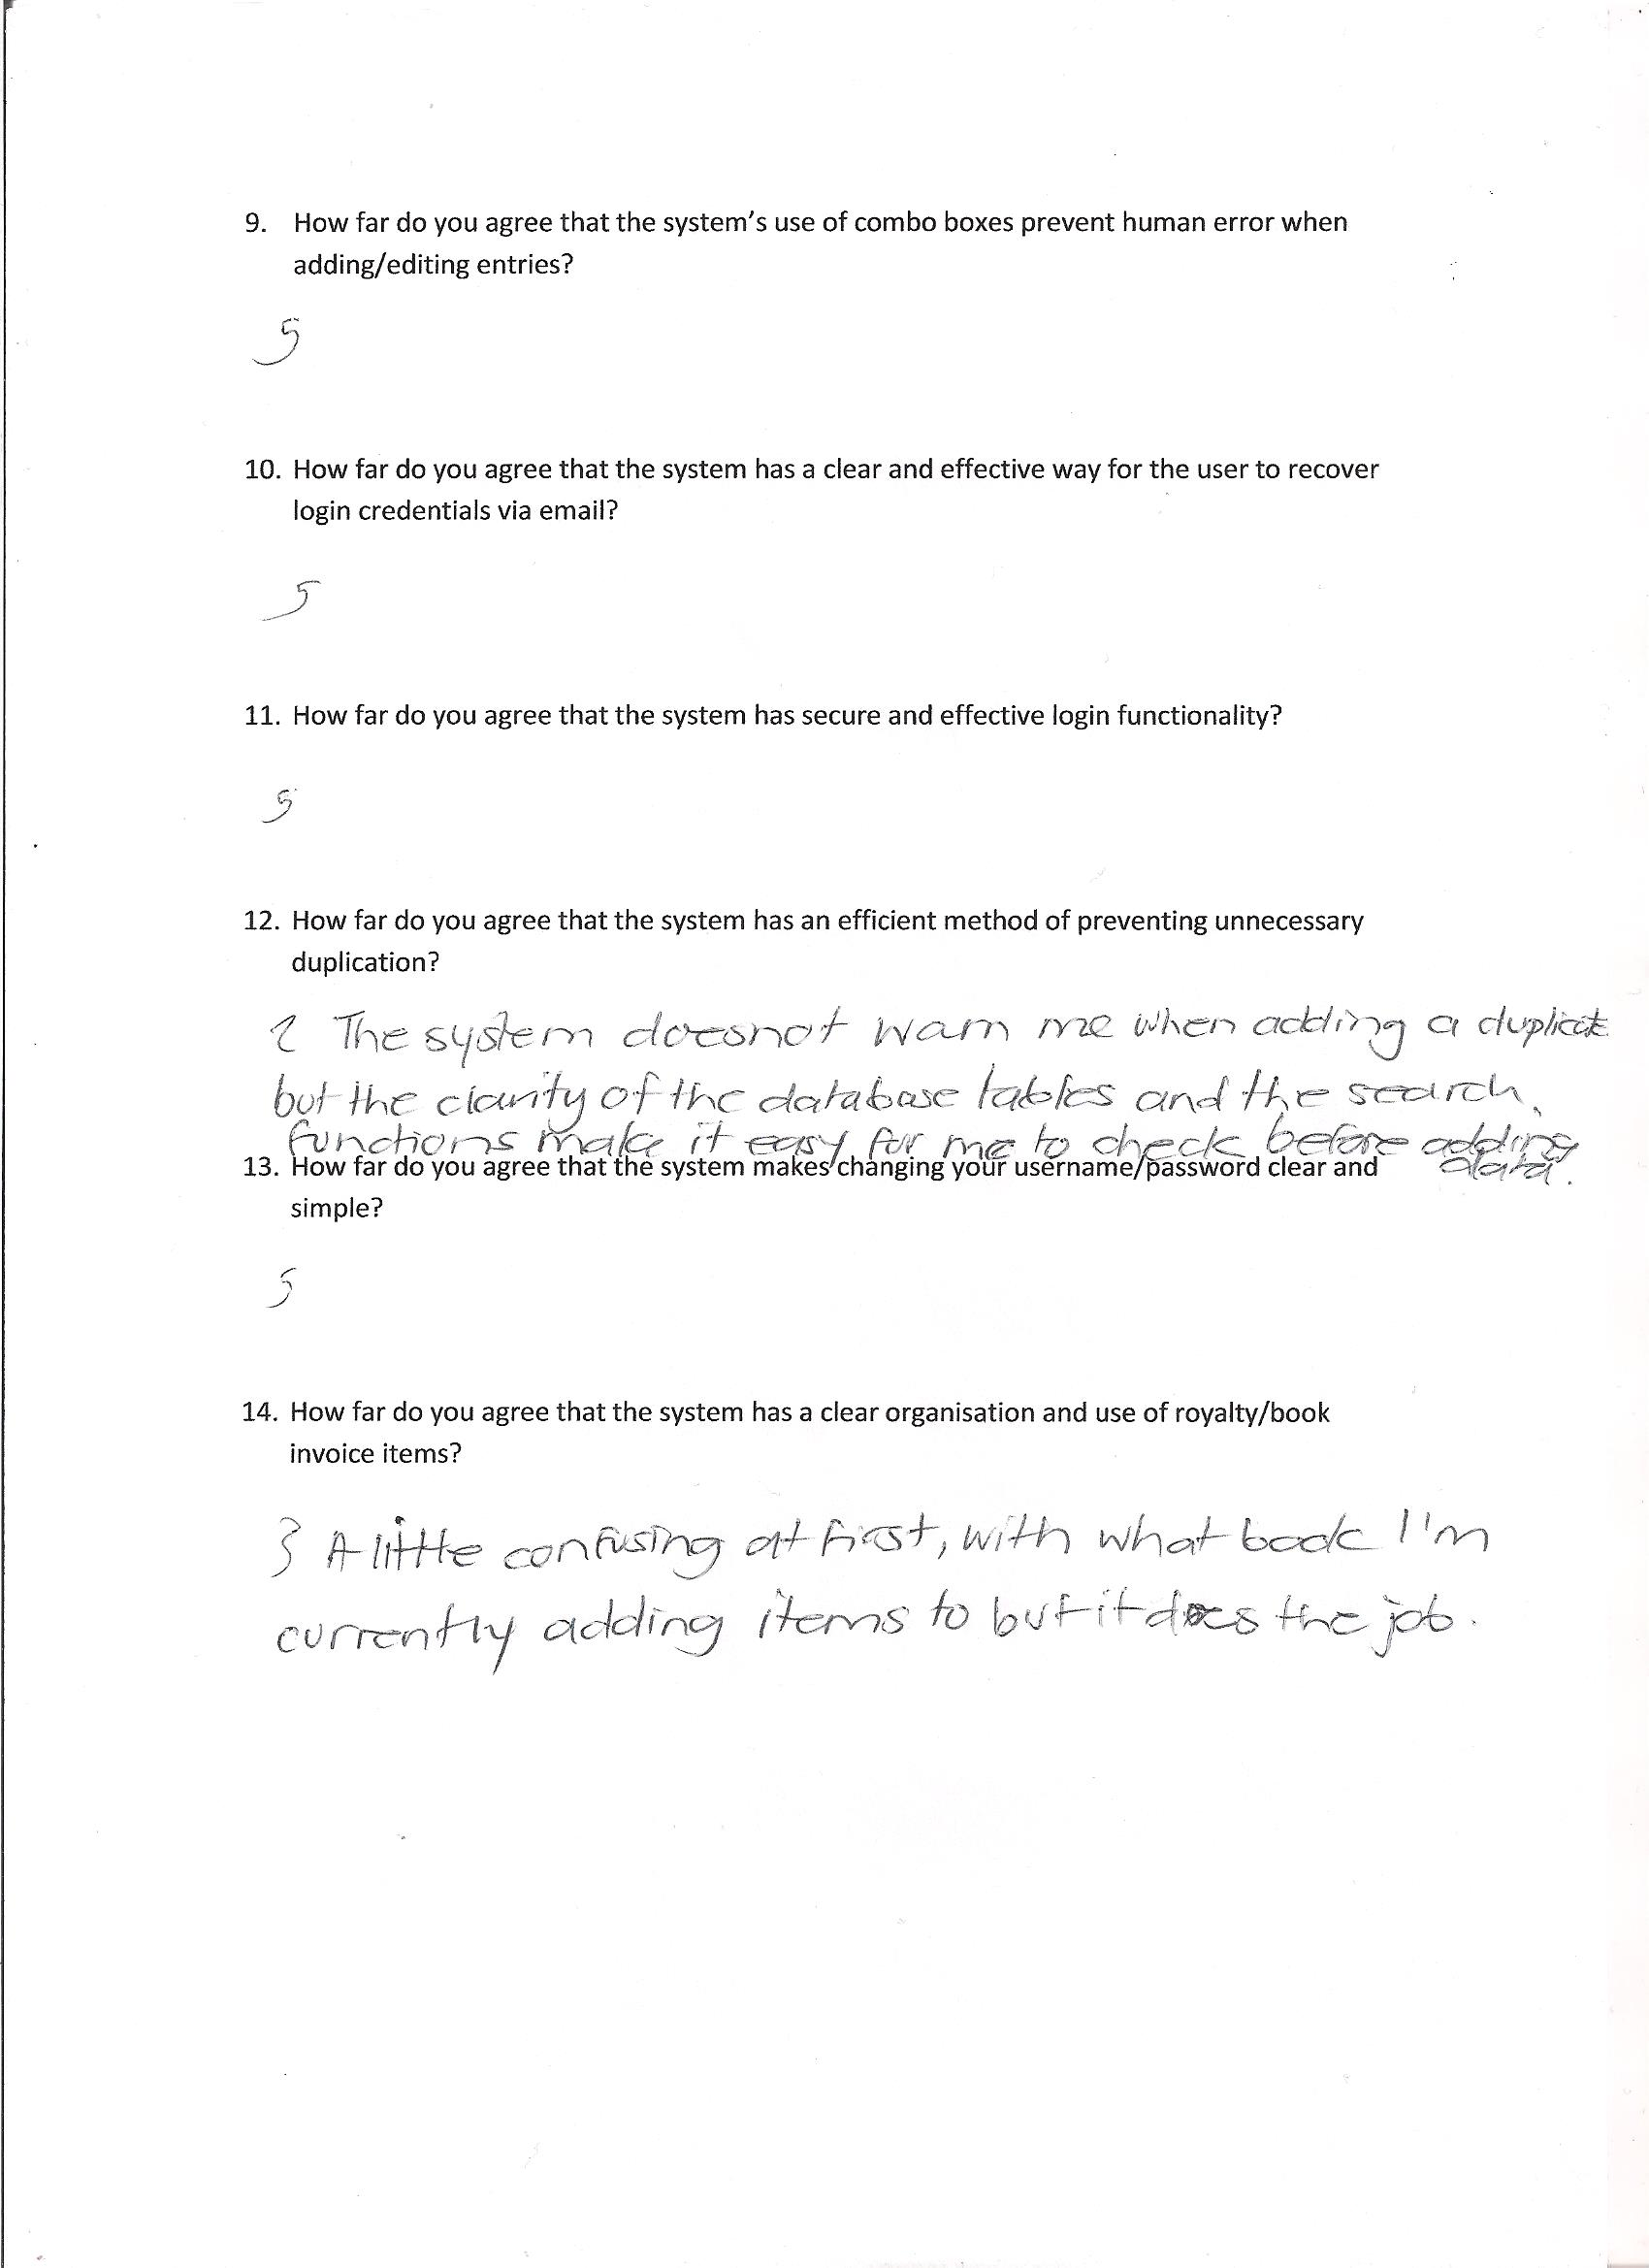
\includegraphics[width=\textwidth]{./Evaluation/Questionnaire2.png}
    \label{fig:QuestionnairePage2} \caption{Page 2 of Questionnaire}
\end{figure}

\subsection{Graphs}

\subsection{Written Statements}
